\chapter{Pulse Oximeter (2B)}

\section{Background}
Hemoglobin is a protein in red blood cells that reacts to oxygen forming oxyhemoglobin (HbO$_2$).  When not oxygenated hemoglobin is referred to as deoxyhemoglobin (Hb).  Pulse oximetry is a non-invasive way to measure the amount of oxygen dissolved in the blood, which is called the oxygen saturation (SpO$_2$). Oxygen saturation is measured by detecting Hb and HbO$_2$, using their absorption sectra at two different frequencies (typically red around 660nm and infrared around 840nm to 940nm).  These values were selected because Hb has higher absorption of red light and HbO$_2$ has higher absorption of infrared, see figure~\ref{fig-spectrum}.

 \begin{figure}
 \caption{Absorption spectra of oxyhemoglobin and deoxyhemoglobin. \emph{Image by Adrian Curtin used under  Creative Commons Attribution-Share Alike 3.0 Unported License.}}
 \label{fig-spectrum}
 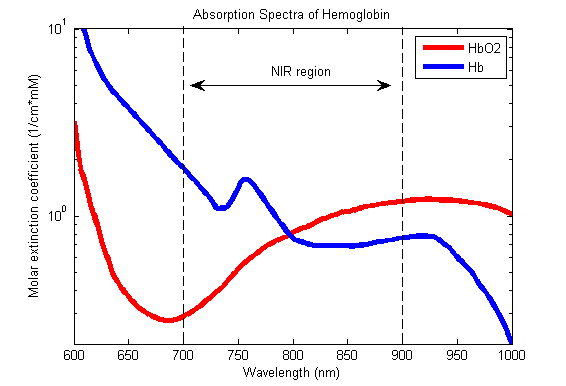
\includegraphics{../images/Oxy_and_Deoxy_Hemoglobin_Near-Infrared_absorption_spectra.png}
 \end{figure}

We are going to use two LEDs, one red one infrared, a photodiode, and a simple filter/amplifier to measure the absorbed light at two frequencies.  The data that produced the graph came from the tabulated molar extinction coefficient, e, for hemoglobin in water compiled by Scott Prahl using data from
\begin{itemize}
\item W. B. Gratzer, Med. Res. Council Labs, Holly Hill, London
\item N. Kollias, Wellman Laboratories, Harvard Medical School, Boston
\end{itemize}

\begin{tabular}{lrr}
$\lambda[ nm]$  & $HbO_2[ cm^{-1}/M]$ & $Hb[ cm^{-1}/M]$ \\
660              & 319.6                  & 3226.56 \\
830              & 974                    & 693.04 \\
840              & 1022                   & 692.36 \\
930              & 1222                   & 763.84 \\
940              & 1214                   & 693.44 \\
\end{tabular}

To get absorption, you multiply the molar extinction coefficient times the molar concentration times the pathlength and divided by the molecular weight of hemoglobin.  Since we are comparing two absorption measurements at different frequencies, the molecular weight of hemoglobin cancels and can be ignored.  Similarly, if we put both light sources (red and infrared) equally distant through your body to the photodiode, then the pathlength will also cancel and can be ignored.  %Let $x_{Hb}$ and $x_{HbO_2}$ be the concentration of deoxyhemoglobin and the concentration of oxyhemoglobin respectively, then the absorption is

Light is absorbed by tissue, venous blood, non-pulsatile arterial blood, and pulsatile arterial blood.  The first three are constant and will be measured as the DC component of the measurements.  The final one, pulsatile arterial blood, will be the AC component, and will also allow us to get heart rate.

\section{First Method}

By taking the ratio of oxygenated arterial blood in the pulsatile (AC) over the other (DC) portion of the signal at two frequencies we can calculate the absorption ratio (AR)\footnote{$SpO_2$ can also be calculated by ratio of the logarithms of the AC components at the two frequencies.  Multiply by 100 to get percent.}
\begin{equation}
AR = \frac{\frac{AC_{red}}{DC_{red}}}{\frac{AC_{infrared}}{DC_{infrared}}}
\end{equation}
We can then compare this number to previously measured values that were tested in a different manner.  This is only approximate because of differences in blood volume, perfusion, etc. as well as movement and misplacement effect measurements.  Even so we can make a simple table of values and interpolate to get other values:

\begin{tabular}{lr}
$AR$ & $SpO_2$ \\\hline
0.4  & 100\% \\
1.0  & 85\% \\
3.4  & 0\% \\
\end{tabular}

